\label{ch::hardware_and_design}
%%%%%%%%%%%%%%%%%%%%%%%%%%%%%%%%%%%%%%%%%%%%%%%%%%%%%%%%%%%%%%%%%%%%%%%%%%%%%%%%%%
%%% Robot Hardware and Design
%%%
%%% Section 1 : Robot Design
%%% 
%%% Section 2 : Controller Configuration/Descriptions
%%%
%%% Section 3 : Sensors
%%%
%%% Section 4 : Device Connectivity Layout
%%%
%%% Section 5 : System Power
%%%		SubSection 5.1 : Power Requirements and Runtime
%%% 	SubSection 5.2 : Power Routing
%%%
%%%%%%%%%%%%%%%%%%%%%%%%%%%%%%%%%%%%%%%%%%%%%%%%%%%%%%%%%%%%%%%%%%%%%%%%%%%%%%%%%%
\chapter{Hardware and Design}


	\section{Overview and Design Goals}
	
	The BlueFoot quadruped robot is designed as a small-scale, general-purpose legged mobile platform with enough physical dexterity and on-board computational/sensory power to perform complex tasks in variable environments. BlueFoot's hardware configuration is aimed at performing of tasks as a standalone unit, i.e. without power tethering or off-board processing. BlueFoot's sensory, computational and power-source outfit make it fit to complete tasks in both settings fully and semi-autonomous modes.

	The implementation of a legged robot which meets these general specification is inherently bottlenecked by several well-known shortcomings which plague legged robot design. These drawbacks can be summarized as follows: relatively low payload capacity, as leg joints are often subjected to substantial dynamic torque loading during gaiting; and higher power consumption due to a, typically, larger number of total actuators. Thus, a general-purpose, multi-legged system like the BlueFoot platform must ultimately achieve a balance between payload-carrying capacity (i.e. maximum joint-servo output torque); actual on-board payload; and on-board energy supply. It is desirable that the sensory and computational power; as well as overall mobility of a legged system are simultaneously maximized along with the aforementioned characteristics. 
	
	The design goals which have guided the implementation of the BlueFoot quadruped have been tailored to a yield an overall system design which is both feature rich, computationally powerful, and exploits the natural dexterity and terrain handling of legged robotic systems. Namely, the core design requirements which have guided BlueFoot's development can be summarized as follows:
		\begin{itemize}
			\item{The use of legs with joint redundancy for improved dexterity}
			\item{The use of smart servos for extended joint feedback and control}
			\item{A distributed on-board and computing architecture for hierarchal task handling}
			\item{A vision sensor array including a camera and laser-ranging sensors}
			\item{30+ minutes of total battery life}
		\end{itemize}
	
	This chapter will outline how an implementation meeting these design goals is achieved, starting with the structural layout of the system. Next, major system payloads and the associated interfacing of major devices will be described. This section which will include details about BlueFoot's actuators, computational modules, and sensory mechanisms. Lastly, the system power routine, energy requirements, and runtime will be detailed.

		\begin{figure}[h!]
			\centering
			\fbox{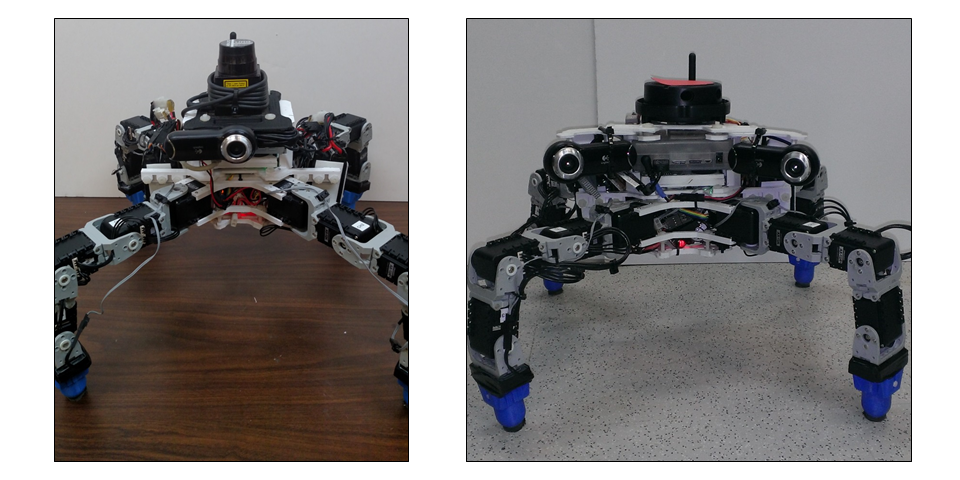
\includegraphics[width=\textwidth]{robot_selfies.png}}
			\caption{The BlueFoot Quadruped Robot: single-camera configuration \emph{(left)}; stereo-camera configuration \emph{(right)}}
			\label{fig::bluefoot}
		\end{figure} 
	
	\section{Robot Structure}
	
		BlueFoot's body is designed in a modular fashion and is comprised of mostly custom designed, 3D printed parts. The use of 3D printing as a fabrication method allowed for rapid design iterations the early stages of system prototyping, and has kept the weight of the robot's overall structure relatively low. Parts were mainly printed from both PLA and SLA plastics. BlueFoot's overall weight (when fully outfitted) is $1.85-1.98 \text{ kg}$, depending on configuration.

		The modularity of BlueFoot's overall structure arises from the inherent design requirements associated with 3D printing and general design practices aimed at keeping the system reconfigurable for the incorporation of updated sensory and computational hardware. Moreover, parts are designed to fit future replacements while conforming to the constraints imposed by the 3D printing fabrication method, i.e. particular part size and orientation requirements. Such constraints had to be met by each designed part to ensure print feasibility. 

		The BlueFoot platform has undergone several minor redesign phases since its inception. These redesigns were necessary to bring the BlueFoot platform to its final structural and hardware state and were performed to accommodate changes in  sensory/computational hardware. The sections that follow will mainly focus BlueFoot's final hardware configurations.

		\subsection{Main Body (Trunk) Design}
		
			BlueFoot's trunk consists of the three main sections: a lower module which interfaces the legs with the main body; a center chassis, designed to  hold computational and battery payloads; and a top platform, which interfaces the system's visions sensors to the trunk. These sections will be referred to as the \emph{Root} module, the \emph{Main} module, and the \emph{Head}module, respectively. The full trunk (not including sensor dimensions) fits within a 21.6 by 21.6 by 15.3 cm bounding box. 

			\subsubsection{The Root Module}

				\begin{figure}[h!]
					\centering
					\fbox{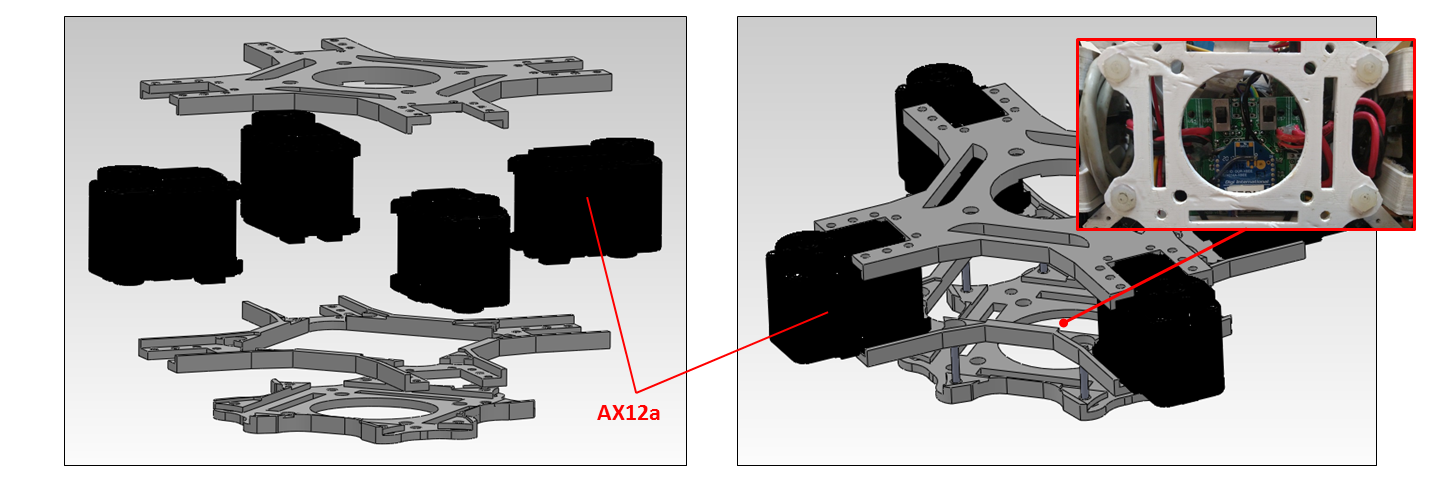
\includegraphics[width=\textwidth]{root_full.png}}
					\caption{Root section of trunk. Call-out in top-right shows main-switch access through the bottom of the root module.}
					\label{fig::root_module}
				\end{figure}

				The Root module, consists of three plates, as shown in Figure~\ref{fig::root_module}. Each plate is designed with a central opening to allow for wired connections to pass to other trunk modules. Two such plates directly interface with four servos, which are mounted to four symmetric arms which extend from the center of each plate. These servos are the first joint (hip-joint) of each leg. Each servo mounts to the top a bottom plates via mounting holes located at the top and underside of each servo chassis. The assembly is mated with small steel bolts. A third, smaller plate is attached to the bottom of the module to provide more space for power components and associated wiring. This plate is attached to the bottom of the module via plastic standoffs. An opening in the middle of this plate provides access to the system's main power switches, as well as a removable XBEE wireless radio unit.

			\subsubsection{The Main Module}
		
				The Main module of BlueFoot's trunk includes compartments for an in-house designed AutoPilot unit and a main computer unit, an ODROID-XU. The Main module is designed such that the AutoPilot and ODROID-XU computer slide in and out of the body. The computer payloads are locked into position when the Head module is added to the assembly. The Main body section is designed to fit both computers when stacked upon one another, as depicted in Figure~\ref{fig::main_module}. The computer stack is positioned directly in the center of the module when inserted.
%
				\begin{figure}[h!]
					\centering
					\fbox{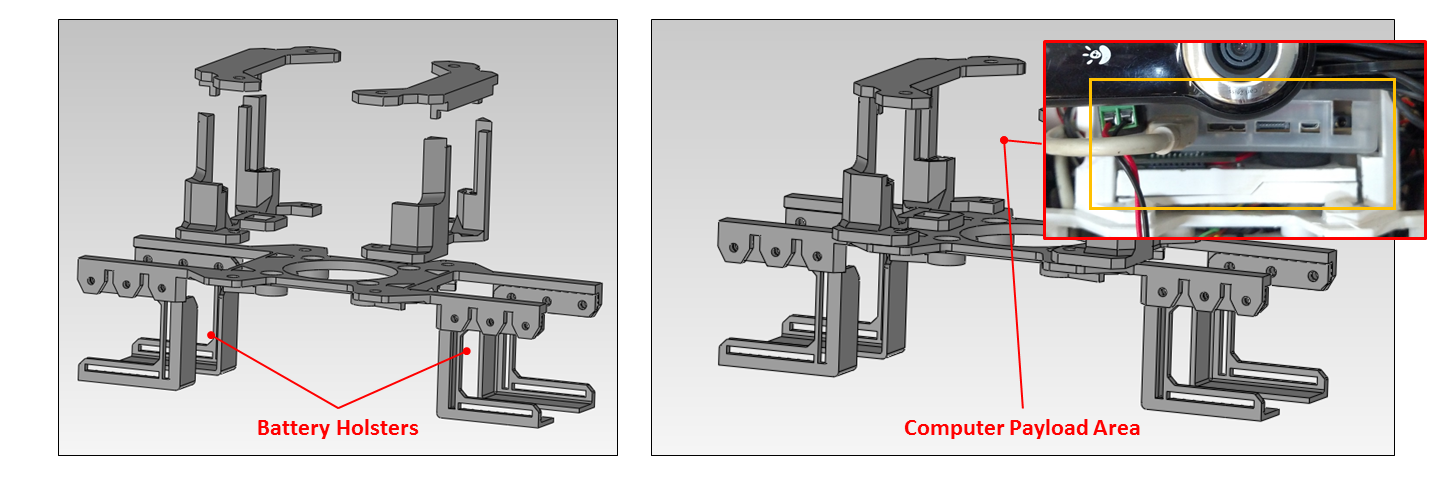
\includegraphics[width=\textwidth]{main_full.png}}
					\caption{Main section of trunk. Call-out in the top-right shows how the ODROID-XU and AutoPilot computers fit within the module.}
					\label{fig::main_module}
				\end{figure}

			
				The Main module also includes two battery holsters, which hang over its left and right sides. The holsters align the battery packs with the center of Root module. This battery placement serves to lower the center of mass (COM) of the trunk. Doing so serves to lower the magnitude of dynamic torques imparted upon the leg servos during gaiting by decreasing the net moment due to gravity imparted upon the system when the body is oriented away from the direction of gravitational force. The entirety of the Main module is attached to the Root module through the battery holster sub-assembly by four plastic bolts.
		
			\subsubsection{The Head Module}

				Two separate Head modules have been designed for the BlueFoot system : one of which features a stereo camera pair and a Piccolo LIDAR sensor (PLDS); and a monocular design, which features a camera and a Hokuyo-URG LIDAR sensor, as shown in Figure~\ref{fig::head_module}. Each head module is attached to Main module via four plastic mounting screws. In the stereo-camera design, two adjustable wings are attached to either side of a top platform which hold cameras. These wings were designed to be adjustable to aid in stereo-camera configuration and calibration. The position of each camera on the trunk allows for a persistent field of view by each camera during mobilization. The PLDS unit is positioned such that the center of its rotating laser head is aligned to the center of the trunk. 

				\begin{figure}[h!]
					\centering
					\fbox{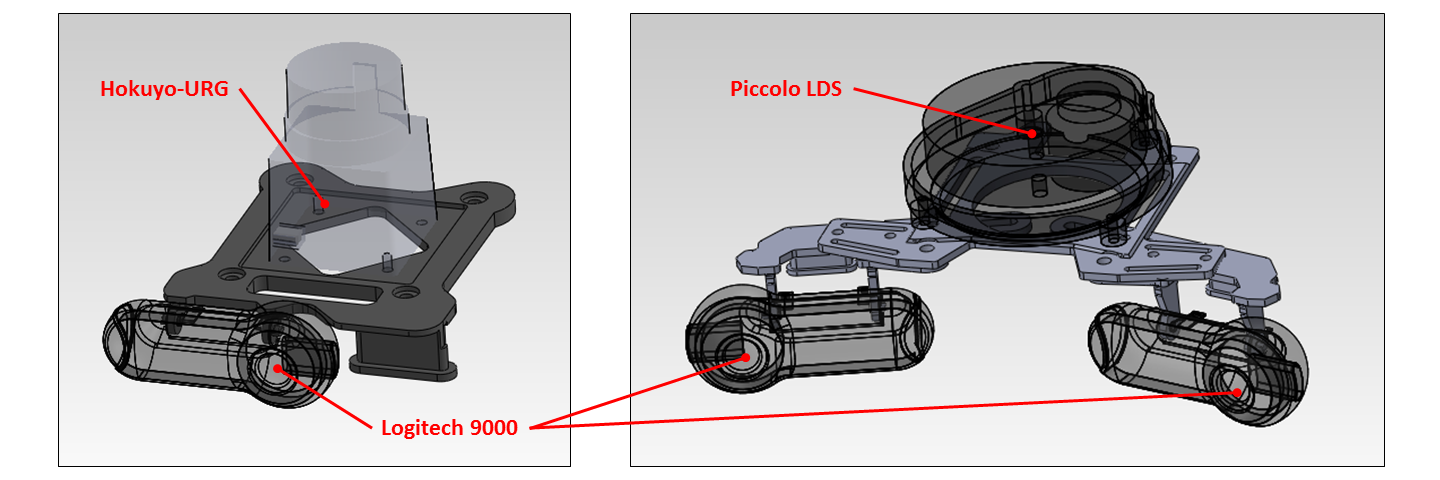
\includegraphics[width=\textwidth]{head_full.png}}
					\caption{Head section of trunk. Monocular camera configuration with Hokuyo-URG \emph{(left)}; and Stereo configuration with PLDS \emph{(right)}. }
					\label{fig::head_module}
				\end{figure}		

				In the monocular design, a single camera is mounted such that the lens of the camera is aligned to the sagittal plane of the trunk. This configuration is currently be used as BlueFoot's \emph{primary} head configuration and is mainly being used for 3D point-cloud building and surface reconstruction via 2D LIDAR scans. This is because the Hokuyo-URG laser scanner used in this configuration offers higher-resolution laser-scan outputs, which will be covered in more detail later in this chapter.

		\subsection{Leg Designs}

			\begin{figure}[h!]
				\centering
				\fbox{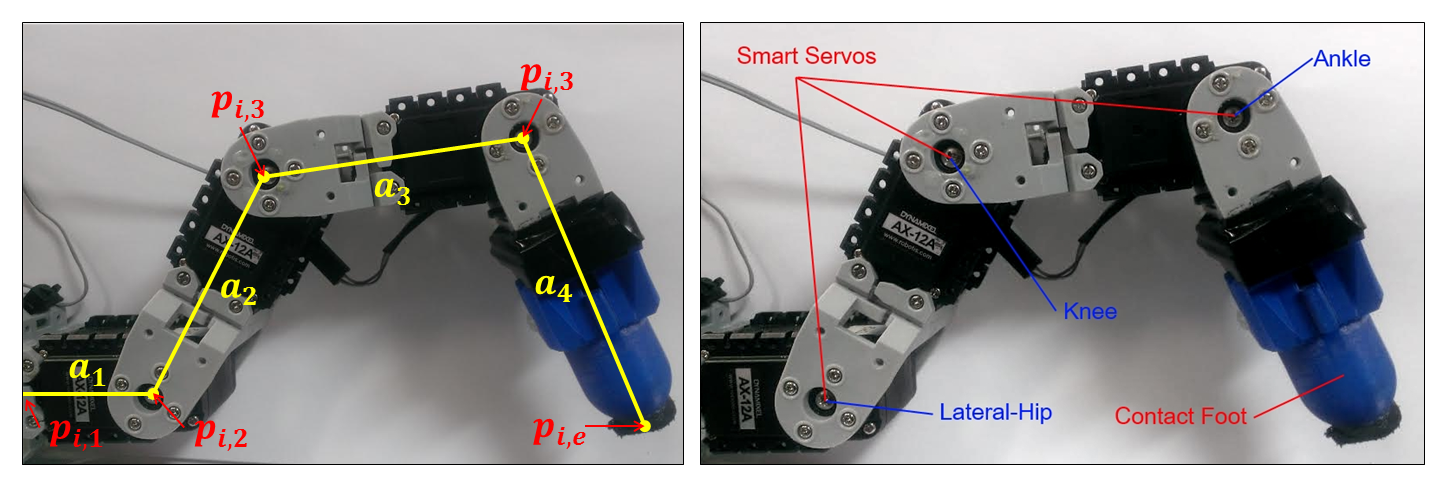
\includegraphics[width=\textwidth]{leg.png}}
				\caption{Closeup of BlueFoot's leg. \emph{(left)} shows effective link lengths and the location of defined joint positions.}
				\label{fig::leg_labeled}
			\end{figure}
				
			Each of BlueFoot's legs are identical and are comprised of four Dynamixel AX12a smart-servo actuators (see Figure~\ref{fig::leg_labeled}). These actuators are connected via dedicated Dynamixel mounting brackets. Feet are attached to the ends of each leg which contain an embedded, two-state contact sensors. Each foot is designed with a spherical tip, which is rubberized to provide extra grip. The ankle joint of the platform has been added such that the platform can reconfigure its foot orientation while retaining a constant spatial position during gaiting. Additionally, this configuration allows for a considerable amount of independent body re-orientation and repositioning. This capability extends itself to the stabilization and gimbaling of vision sensors mounted on the upper body of the platform while the platform is in motion.
		
			\begin{figure}[h!]
				\centering
				\fbox{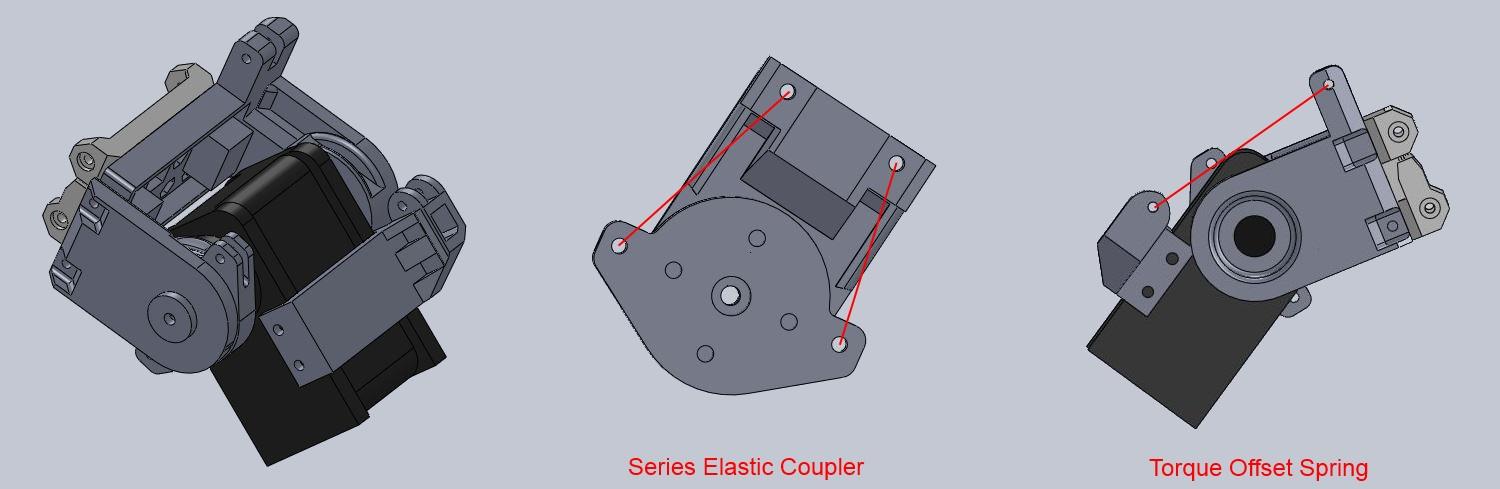
\includegraphics[width=\textwidth]{sea_full.jpg}}
				\caption{Series elastic brackets.}
				\label{fig::sea_bracket}
			\end{figure}

			Though not kept in the system's final design, some experimentation was performed with the incorporation of series elastic joints, which were designed to relieve joint impact during gaiting. Series elastic actuation was achieved by replacing bracket interfacing the first and second hip joints of each leg with an elastic-compliant mounting bracket. This bracket includes spring loaded member which was mounted to the horn of the second hip servo on each leg, as shown in Figure~\ref{fig::sea_bracket} and allowed the leg to deflect a small amount at the lateral hip (second joint).

			Link lengths, $a_{1}, a_{2}, a_{3}$ and $a_{4}$; and offset from the center for the Root module to the first joint of each leg, $\nu$, are defined in Table~\ref{tab::link_lens}. These parameters are identical for each leg, and are corresponded with physical leg members labeled in Figure~\ref{fig::leg_labeled}.

			\begin{table}[h!]
				\centering
				\begin{tabularx}{\textwidth}{|C{0.5}|C{0.5}|} 	
					\hline
					\bf{Link} 	&	\bf{Length, m}	\\	\hline \hline
					$a_{1}$ 	&	0.06500			\\	\hline
					$a_{2}$		&	0.06500			\\ 	\hline
					$a_{3}$		&	0.06500			\\ 	\hline
					$a_{4}$		&	0.06500			\\ 	\hline
					$\nu$		&	0.09215			\\	\hline
				\end{tabularx} 
				\caption{Link and body-offset lengths for each leg.}
				\label{tab::link_lens}
			\end{table}


	\section{Computational and Sensory Hardware}
		
		\noindent
		Major payloads on-board the BlueFoot robot are as follows: 

			\begin{itemize}
				\item{Dual processor AutoPilot unit with a 12-axis inertial measurement unit}
				\item{ODROID-XU Computer}
				\item{Logitech 9000 Web-cameras}
				\item{Hokuyo-URG / Piccolo LIDAR Units (configuration dependent)}
				\item{Two-state foot contact sensors (x4)}
				\item{Dynamixel AX12a Smart Serial Servos (x16)}
				\item{XBEE Wireless radio}
			\end{itemize}

		Device selection has remained mostly consistent since the platform's inception and initial design, with the exception of computing its main computing units. The AutoPilot unit was updated from an older model, and the ODROID-XU computer replaced a Beaglebone computer for the sake of improving overall computing power.

		\subsection{Device Descriptions}
	
			\subsubsection{AutoPilot}

				A dual processor AutoPilot unit performs BlueFoot's low-level gaiting and actuator control tasks, as well as handles communications with a computer running ground-station software. Given the set of low-level sensory and motor-handling tasks it performs, this module has been named the the ``Lower Brain" (LB) of the system. The AutoPilot consists of two processing units: a TM4C and RM48 micro-controller (MCU), which operate at 80 MHz and 220 MHz, respectively. These processors communicate over a single UART line, which is used to transfer packeted data between the two processors using a unified inter-processor data transfer protocol, EXI. This protocol which will be described later in more detail. One UART of the RM48 MCU is also connected to an on-board computer, an ODROID-XU, through a USB-to-serial connection. The AutoPilot is powered via an external 12 V supply.
	
				This AutoPilot unit includes a 12-axis inertial measurement unit (IMU) which consists of two, 3-axis accelerometers; one 3-axis rate gyro; and a 3-axis magnetometer unit. This sensor is used for acquiring angular rate data of BlueFoot's trunk and estimating of trunk orientation states using an Extended Kalman Filter (EKF). 
				
			\subsubsection{ODROID-XU}

				An ODROID-XU performs many of system's high-level planning tasks, such as navigation, image processing and terrain reconstruction; and handles data data acquisition from both camera and LIDAR sensor units. Given that this unit performs mostly high-level planning tasks, it has been given the name ``Upper Brain" (UB). This computer contains a 1.6 GHz, quad-core processor with 2 Gb of RAM. The ODROID-XU can be communicated with over WiFi via a USB WiFi antenna. Currently, SSH tunneling is used to start processes on the ODROID remotely and stream data. The ODROID-XU is powered via an external 5V connection.

			\subsubsection{Logitech 9000 Web Cameras}

				Logitech 9000 web cameras have been selected for creating a stereo camera pair, as well as for use in a single camera configuration. These cameras are high-definition web cameras and have a maximum frame rate of 30 fps and a max resolution of 1280 by 720. Cameras are currently read at a the max rate of 30 fps at a more conservative resolution of 640 by 480. These settings are adequate for image processing tasks and have been chosen to reduce nominal data throughput. These cameras are interfaced with the UB (OROID-XU) over a USB connection.

			\subsubsection{Laser Distance Sensors (PLDS and Hokuyo-URG)}

				The Piccolo Laser distance sensor (PLDS), which is used in BlueFoot's stereo-camera type configuration, is a 4 meter spinning-head laser range finder. The PLDS has a resolution of a point per degree and covers a range of 360 degrees. Ranging frames (which covers a full rotation) are acquired at a rate of 5 Hz, and are dispatched over a serial connection at 115200 baud. An FTDI break-out board is used to convert the sensor's raw serial output to USB protocol so that the sensor can be interfaced with the UB unit. The PLDS is powered via and external power 5 V source, which is regulated to a 3.3 V voltage level for powering the motor which spins the laser head, and 1.8 V for internal logic. Regulation is performed by an auxiliary power circuit.

				The Hokuyo-URG Laser Distance sensor, which is used in BlueFoot's single-camera head configuration, has a a range of 5.6 metets and an angular resolution of 0.38 degrees per point (628 points per scan). This scanner covers a total angular range of 240 degrees. Ranging frames are acquired at a rate of approximately 10 Hz and dispatched directly over a USB connection at 115200 baud. The unit is powered directly over USB.

			\subsubsection{Foot Contact Sensors}

				Binary-state contact sensors are embedded in each foot. These contact sensors are essentially limit-switches which generate an active-low signal when the foot comes in contact with the ground. Each sensors is connected to ground and a GPIO pin on the TM4C MCU of the AutoPilot. A 500 $\Omega$ is added in series with the limit-switch for the purpose of pin protection.

			\subsubsection{Dynamixel AX12a Smart Serial Servos}

				BlueFoot uses 16 Dynamixel AX12a servo units (4 per leg). These servos are position-controlled and commanded over a daisy-chained, half-duplex serial bus (i.e. single wire) at a rate of 1 Mbps. These servos have a maximum holding torque of 1.618 N m and top speed of 306 degrees/s. The AX12s provide position, velocity and loading feedback, however velocity feedback is not used. Servo velocities are, instead, estimated in real time from position feedback because velocity readings provided by the AX12 is relatively noisy by comparison. 

				Commands are sent to the servos via an aggregate command packet which contains goal-position values for all servo units. Feedback is collected from each servo using individual data-request packets. Servos respond to each request with a response packet containing a corresponding feedback value. Given the number of servos in the network; communication overhead; and the one-wire communication configuration, servo updates are limited to a maximum update rate of 50 Hz over a half-duplex communication line. Gathering feedback over the half-duplex communication bus is particularly expensive because feedback requests require that the host processor wait after each dispatched for a response from each targeted servo. Moreover, each request/response cycle must finish to completion before a feedback request is made to another servo on the communication bus.

				A dedicated circuit has been designed for use with these servos which converts a full-duplex serial line to a half-duplex AX12 bus. The circuit uses a two-state tri-state buffer which is switched via a general-purpose I/O line. This switching circuit is integrated into the system's main power switching and distribution board. Each servo is powered via an fused, software-switched 12 V supply line.

			\subsubsection{XBEE Wireless Radio}

				An XBEE Wireless Radio, shown in Figure \Markup{This could be the picture from before}, is used for communication between the LB and an external computer ground-station. The radio is interfaced with the LB via 57600 baud serial connection. This radio has a range of outdoor range of 27 meters and a maximum one-way transfer-rate of 115200 bps. Transfer rates between the LB and ground station are currently being limited to 57600 bps to compensate for a lack of hardware flow-control, which is required for stable, two-way communication between two XBEE radios at maximum communication rates. However, the selected communication rate is more than adequate for transferring necessary control information to and from the system without the need for additional flow-control hardware.

				This wireless endpoint is used currently used interchangeably with the ODROID-XU's wireless WiFi radio, but will soon be retired to simplify hardware design and increase the platform's data streaming capabilities by switching to a WiFi-based line of communication. Ground station software, as well as the system's internal command-routing and networking software, is designed in such a way to easily accommodate this change.

		\subsection{Device Networking}

			\begin{figure}[h!]
				\centering
				\fbox{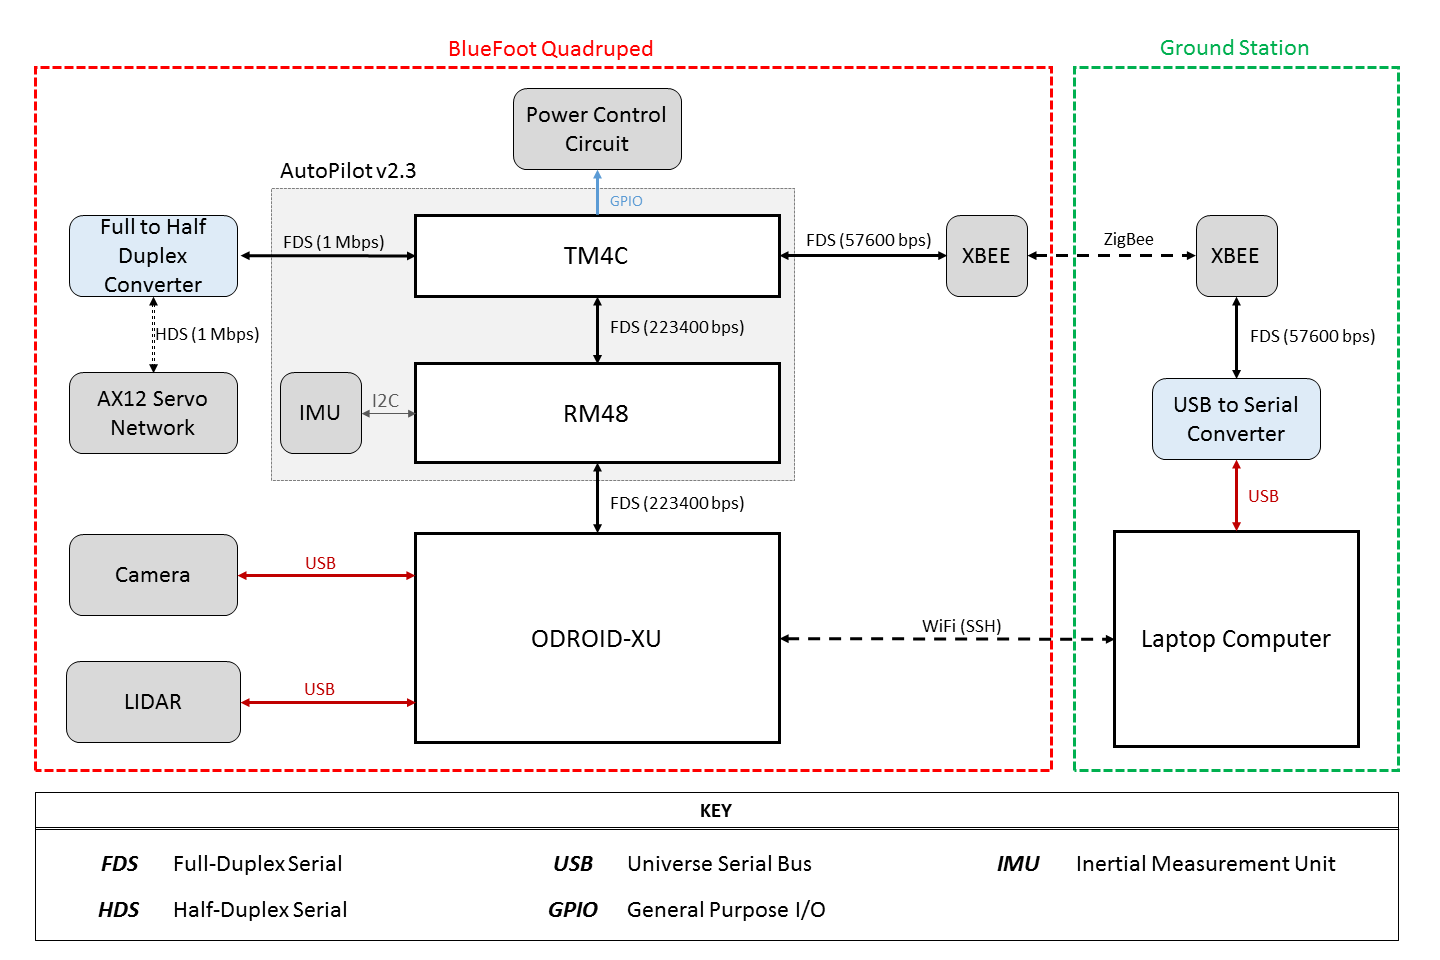
\includegraphics[width=\textwidth]{device_diagram.png}}
				\caption{BlueFoot device networking diagram.}
				\label{fig::dev_diagram}
			\end{figure}
			
			
			Figure~\ref{fig::dev_diagram} depicts how each major device is connected within the system and details the communication rates ($f_{com}$) between networked devices. Accompanying specifications are detailed in Table~\ref{tab::comm_port_pairs}, which summarizes all device communication pairs and their corresponding baud rates.

			\begin{table}[h!]
				{\footnotesize XBEE$^*$ refers to the on-board XBEE module which communicates with the ground station.}
				\centering
				\begin{tabularx}{\textwidth}{|C{0.2}|C{0.2}||C{0.2}|C{0.2}||C{0.2}|} 	
					\hline
					\bf{Port$_A$} &	\bf{Source$_A$}	&	\bf{Port$_B$}& 	\bf{Source$_B$}	& 	\bf{$f_{com}$, kbps}\\	\hline \hline
					UART0 		&	TM4C			&	DIN/DOUT	&	XBEE$^*$		&	55.7 				\\	\hline
					UART2		&	TM4C			&	DIN+		&	AX12 Net.		&	1000				\\ 	\hline
					UART1		&	TM4C			&	LINSCI		&	RM48			&	223.4				\\ 	\hline
					SCI			&	RM48			&	USB (FTDI)	&	ODROID-XU		&	223.4				\\ 	\hline
					USB			&	ODROID-XU		&	DIN/DOUT 	&	LIDAR 			& 	115.2				\\	\hline
					USB			&	ODROID-XU		&	USB			&	Cameras	 		& 	No Spec.			\\	\hline
				\end{tabularx} 
				\caption{System communication port-pairs and corresponding data transfer rates}
				\label{tab::comm_port_pairs}
			\end{table}


	\section{System Power}

		\subsection{Power Routing}

			System power routing is handled via an integrated power switching and distribution board. This board includes physical, main power switches which connects external power to two main, internal 12 volt buses for  computer power (Net-1) and motor power (Net-2), respectively. The board also regulates system input voltage to a 5 V bus for use with on-board ICs and 3.3 V bus for powering the XBEE radio. Regulated power and power the servo motors of each leg controlled via three, two-channel power-switching IC's, which are toggled using six digital I/O pins on the TM4C processor of the LB. These power-switching chips allow for software-controlled power configuration, and further, software controlled emergency power cutoff to the servo motors. System main power is supplied via four 12 V (3 cell), 2 Ah Lithium Polymer battery packs.
			%
				\begin{figure}[h!]
					\centering
					\fbox{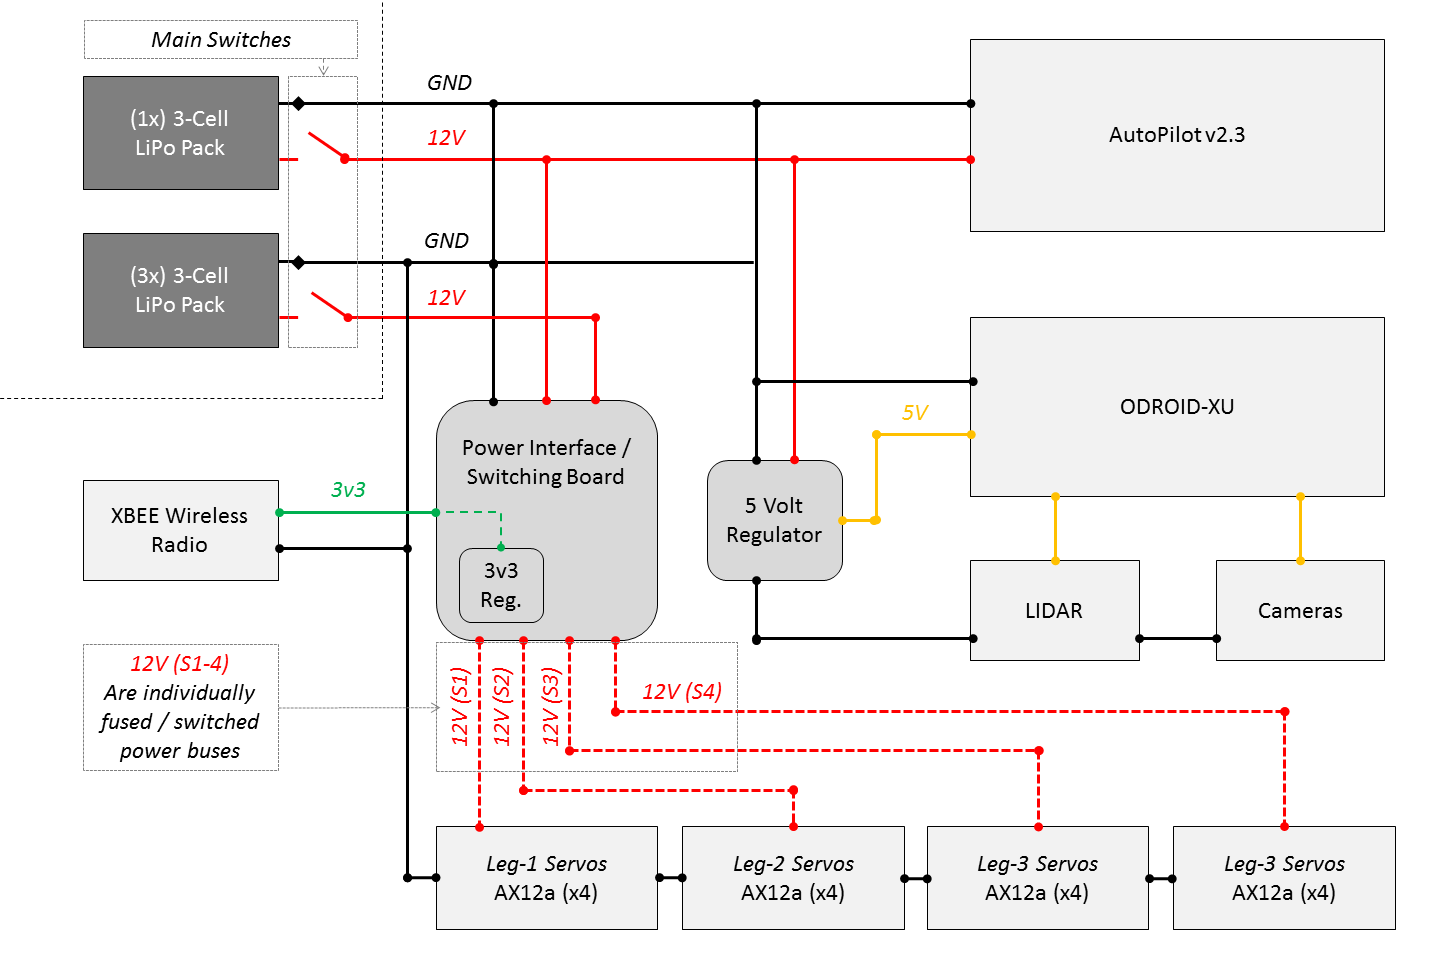
\includegraphics[width=\textwidth]{power_diagram.png}}
					\caption{BlueFoot power routing.}
					\label{fig::dev_diagram}
				\end{figure}
		
			\subsection{Energy Requirements and Runtime}

			
			The power consumptions of BlueFoot's component device's are summarized in Table~\ref{tab::power_summary}, which provides the operating voltage, $V_{op}$, and nominal current draw, $I_{nom}$, of each active, on-board component. Table~\ref{tab::runtime_summary} details battery specifications (output voltage and amp-hour rating) and BlueFoot's estimated run-time under nominal operating conditions.
		
		
			\begin{table}[h!]
				\centering
				\begin{tabularx}{\textwidth}{|C{0.1}|C{0.4}||C{0.25}|C{0.25}|} 
					\hline
					\textbf{Net} 	&	\textbf{Device} 		&	\textbf{$V_{op}, V$}	&	\textbf{$I_{nom}, A$}	\\	\hline\hline
					1				&	AutoPilot (RM48, TM4C) 	& 	12.0					&	0.40	 				\\	\hline
					1				&	XBEE Radio 				&	3.3						&	0.25					\\ 	\hline
					1				&	ODROID-XU 				&	5.0						&	2.0						\\ 	\hline
					1				&	Logitech-9000			&	5.0						&	0.1						\\ 	\hline
					1				&	Hokuyo-URG				&	5.0						&	0.5 					\\	\hline
					2				&	AX12a Servos (x16)		&	12.0 					&	9.6	($~$0.6 ea.)		\\	\hline
				\end{tabularx} 
				\caption{Power consumption summary by device (for single-camera configuration).}
				\label{tab::power_summary}
			\end{table}


			\begin{table}[h!]
				\centering
				\begin{tabularx}{\textwidth}{|C{0.1}|C{0.4}||C{0.25}|C{0.25}|}
					\hline
					\textbf{Net} 		&	\textbf{Battery Pack}	&	\textbf{$V_{out}, V$}			&	\textbf{Rating, $A.hr$}	\\	\hline\hline
					1				&	3S LiPo Pack (x1)		& 	12.0						&	2.0	 					\\	\hline
					2				&	3S LiPo Pack (x3)		&	12.0						&	6.0						\\ 	\hline
				\end{tabularx}

				\begin{tabularx}{\textwidth}{|C{0.5}|C{0.5}|}
					\hline
					\textbf{Total Estimated Runtime}													&	35-40 minutes			\\ 	\hline
				\end{tabularx}
				\caption{Battery power supply and estimated runtime summary.}
				\label{tab::runtime_summary}
			\end{table}